%\subsection{Neocortical Layer 4/5 Pyramidal Cell Test Suite}

%Direct Quote: "widening of the spike shape, decrease of the firing rate and change in the interspike interval distribution". %All these single unit waveform shapes increased their width with temperature.\cite{goldin2017temperature}



%\subsubsection{%\subsection{Section 2.1}
%
%2. Results for several optimized models.
%    2a. First just do basic ones (like Izhikevich) for a few cell types, then you can close with L5PC.
%    2b. The app (which supports 2a).

%\subsubsection{2a}

\section{Performance of Optimized Models}
\subsection{Performance of Layer 5 Prefrontal Cortex Pyramidal Neuron Model on Appropriate Data Driven Tests}

\subsection{Somatosensory Layer 5 Pyramidal Neuron Model Applied to NeuronUnit Tests}

Below I introduce a different approach to parameter fitting work: a multi-compartment, conductance based layer 5 pyramidal cell model \citep{van2016bluepyopt}, was appropriated from BluePyOpt optimization framework, and massaged into the NeuronUnit framework.
This model subserved as one of many component neurons in the priginal formulation of the Blue Brain Project \cite{markram2015reconstruction}.
This elaborate biophysical model is the philosophical opposite of the reduced models focused on in the majority of this thesis work, since the model incorporates electrically complex phenomena instead of excluding it from the model.
The complex model includes a dendritic action potential which can travel ``backwards" from distal dendrite to soma where it is free to summate with incomming EPSPs.
As you can see in the list of parameters (Figure \ref{fig:ca1_parameters}), The model has different adjustable conductance's in 3 out of 4 membrane domains including axons, dendrites, and soma.
There are also other parameters (not displayed here) which are fixed, but those specified in Figure  \ref{fig:ca1_parameters} are amenable to fitting in the context of optimization.


An existing cell from the layer 5 somato sensory rat, hind leg region was acquired by cloning an the BluePyOpt GitHub Repository \cite{van2016bluepyopt}
. Neuroelectro lumps together, prefrontal cortex, somatosensory cortex and V1 PC cells together into a generic frontal cortex pyramidal cell model. 

% Overall it seems

%on NeuronUnit tests of model data agreement}
%\subsection{Section 2.1}
%
%, so it is probably not comparable to NeuroElectro Data.
A suite of neuronunit tests containing the tests: rheobase value, membrane voltage time constant ($\Tau_{m}$), input resistance was computed. This multi-compartment, conductance based model served as a useful benchmark, for us to evaluate the relative performance of reduced model fits. 

%A test suite was constructed using NeuroElectro for the layer 4/5 Prefrontal Cortex pyramidal cell, and we were able to evaluate this layer 5 PC cells against the criteria of the neuroelectro test suite.


Significant development work went into making the model eligible to take NeuronUnit tests, by way of creating a specially dedicated NeuronUnit backend, to run this complicated conductance based multi-compartment model originating from the blue brain model \cite{markram2015reconstruction}. The intention is that by making this model interoperable with NeuronUnit the model will be able to amenable to optimization.


This elaborate biophysical model includes the backpropogating dendritic action potential.
\url{https://github.com/BlueBrain/BluePyOpt/blob/master/examples/l5pc/L5PC.ipynb}
\url{https://github.com/social-hacks-for-mental-health/BluePyOpt/blob/master/examples/l5pc/L5PC.ipynb}


It is possible that the majority neuroelectro recordings of L5PC, spike width were conducted under room temperature as opposed to body temperature, and the relative cooling may have contracted their spike width.
\cite{goldin2017temperature}

\begin{figure}
  \centering
    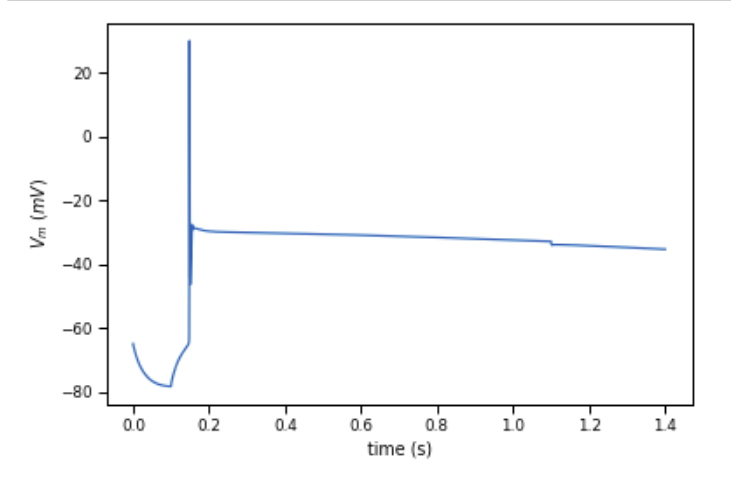
\includegraphics[scale=0.8]{figures/correct_active_l5pc.png}
    \caption[Short duration spike in the L5PC model]{A current injection sufficient for causing a single spike is applied to cell soma, for a whole second from $100ms-1100ms$ in this model. The spike shape is brief and more complicated than reduced model spike shapes. After the very brief spike soma voltage seems to plateau over the entire length of the simulation. The simulation is not long enough for the soma voltage to return to resting membrane potential}
  \label{fig:sub1}
\end{figure}


\centering
\begin{figure}
  \centering
    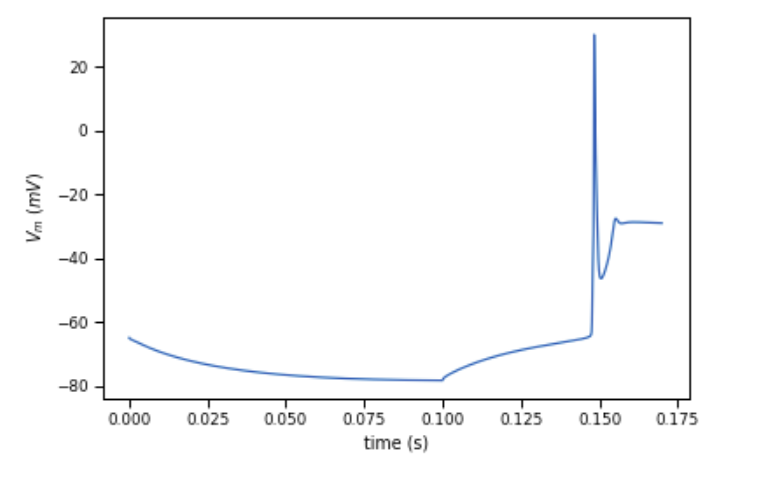
\includegraphics[scale=0.8]{figures/spike_shape.png}
    \caption[Complex spike in the L5PC model]{The above plot warranted a closer look, therefore, this plot features the same model and the same virtual experiment as above, only a smaller time interval has been inflated to fill the whole time axis. In this plot of increased time resolution there is a visible detour in the spikes path to re-polarisation. This unusual feature may be related to a back-propogating dendritic spike, which, a depolarisation wave may have returned from the distal dendrite and has re-invaded the soma, causing the voltage to plateau far above resting membrane potential. These are behaviors, that are obviously neglected in reduced model design}
  \label{fig:sub1}
\end{figure}

\begin{figure}
\begin{center}

    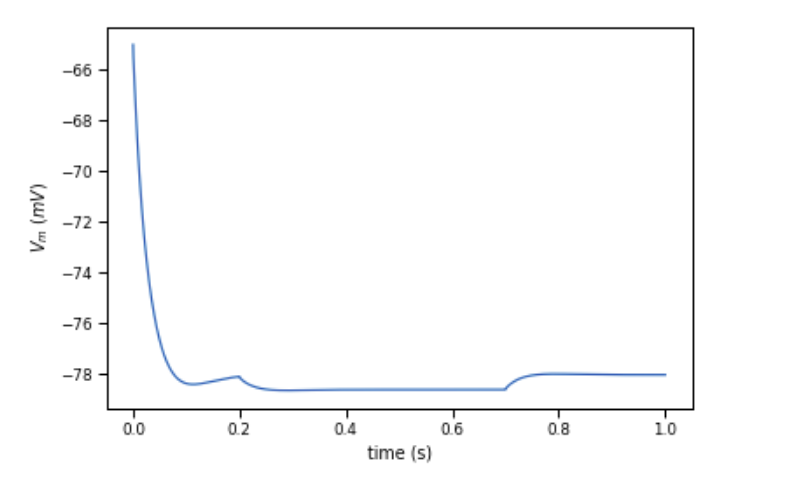
\includegraphics[scale=0.8]{figures/correct_passive_l5pc.png}
    \caption[passive virtual experiment in the Layer 5 Pyramidal Cell]{A current injection value of -$10pA$ is applied to the soma of the pyramidal cell for the duration of $200ms-700ms$. This plot shows the membrane potential at the soma of the multi-compartment model displaying overall expected behavior, the trough of the negative voltage deflection is not as deep as that seen in many reduced models. This suggests the small amplitude of the negative deflection suggests that the L5 PC model is has less resistance than most of the reduced models fitted to the same data, and indeed a low resistance measurement is confirmed in the table below.}
  \label{fig:sub2}
\end{center}
\end{figure}


\begin{table}[ht]
\centering
\resizebox{\textwidth}{!}{
\begin{tabular}{lllll}
\toprule
{} & observations &   predictions & Z-Scores & SEM \\
\midrule
RheobaseTest                   &    213.9 pA &      225.0 pA &  0.065 & 128.9 \\
InputResistanceTest            &  120.7 Mohm &  50.7 Mohm &  -0.90 & 27.9 \\
TimeConstantTest               &     15.7 ms &      16.76 ms &   0.14 & 2.6 \\
CapacitanceTest                &    150.6 pF &     330.7 pF &    1.28 & 1.49 \\
RestingPotentialTest           &    -68.3 mV &     -78.1 mV &   -1.5 & 44.0 \\
InjectedCurrentAPWidthTest     &      1.21 ms &       0.15 ms &   -1.98 & 0.175\\
InjectedCurrentAPAmplitudeTest &     80.4 mV &      89.6 mV &   0.72 & 1.49\\
InjectedCurrentAPThresholdTest &    -42.7 mV &     -59.6 mV &   -2.09 & 1.92\\
\bottomrule
\end{tabular}}
\caption[Z-scores, Observed and predicted features for The Layer 5 Pyramidal Cell]{As the Layer 5 pyramidal cell was made eligible for neuronunit testing. A suite of relevant Neuroelectro L5 Pyramidal cell tests were applied to this cell model iteratively in an optimization framework. This table shows the end result of this process, where agreement between model and experiment has been maximized. The result of the test shows that the model falls within the range of biological plausibility, although model results are far from perfect in all tests. Notably the Rheobase value agrees well with experiments, as does the membrane time constant}
\end{table}
The corresponding statistics were
$(\chi^{2},p_{value})=(13.56, 0.094)$.
Note that the p-value is not sufficiently low to reject the null hypothesis that this model neuron is not from the same distribution as the biological/experimental results.
This may reflect the highly variable nature of the biological/experimental results, rather than the verisimilitude of the optimized model.
Nonetheless, given this experimental variability, the optimization is at least satisfactory. It is also worth noting that not all optimization results lead to the same solution, between different model fitting routines, the optimizer had to choose between fitting the membrane time, constant, fitting the spike width, and fitting the input resistance as the model could be made to fit only one of these measurements at a time. In other words in this model: input resistance, time constant, and spike width were conflicted.


%Hind-limb
%\cite{van2016bluepyopt}
%To understand the validity of model re-purposing, we tested a model constrained on Layer 5 Somatosensory cortex Pyramidal neurons. 

There were two points to this exercise: the first point was to show that multi-compartment conductance based models, are very slow to evaluate, and the second point was, that without enough time, the results are not necessarily as good as you would expect for the inclusion of additional complex mechanisms. There is an unintended straw man character to this observation, it's stipulated in the model documentation (a python notebook) that the model would require a run of at least $100$ generations and a population size of $100$ too properly optimize relative to a different set of constraints. Unfortunately I did not have the time or the computer resources to apply the specified optimization job. However these time considerations bolster a different assertion from my thesis work, timeliness of simulation results aids model refinement, whereby brief simulation times improves scientific insight.

best possible.
However, the model itself happens to be a determing factor in reducing time. The resulting optimized model might serve as a useful benchmark, for us to evaluate the relative performance of reduced model fits. 

A suite of Neuronunit tests containing the tests: rheobase value, membrane voltage time constant ($tau_{m})$, input resistance was computed. 
% somatosensory cortex, or cell from the l5 somatosensory rat, hind leg region, so it is probably not comparable to NeuroElectro Data.

Significant development work went into making the model eligible to take NeuronUnit tests, and amenable to NeuronUnit driven optimization, to make this complicated conductance based multi-compartment model interoperable with the NeuronUnit test judging paradigm.
The intention is that by making this model inter-operable with NeuronUnit the model will be able to amenable to different, optimization. 

\begin{figure}
    \centering
    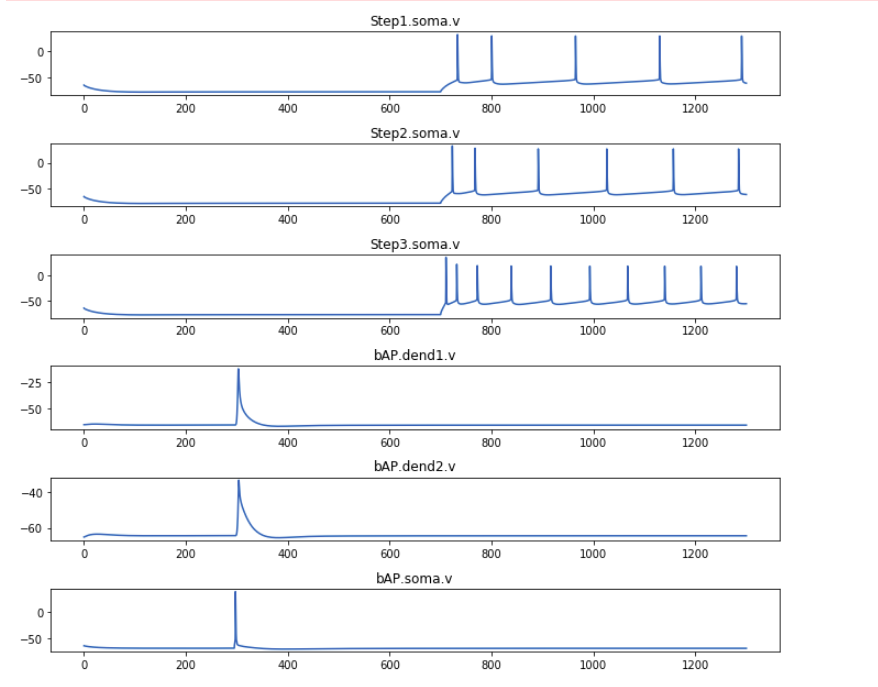
\includegraphics{figures/l5pc_before_opt}
    \caption[L5PC before optimization][Behavior of the L5PC model under default parameters]{Behavior of the L5PC model is explored under three different stimulus strengths. Membrane potential this time is viewed from recording locations in the soma and dendrites. In this recording site at the dendrite there is a singular backpropogating spike. Although the soma and axon hillock, trigger an adapting spike train, lasting more than a second, the dendrite only receives one backpropogating potential, which has a large spike half width. The reason the axon fires multiple times, but the dendrites fire once, is because  dendrites contain dominating passive mechanisms, that can low pass filter invading currents}
    \label{fig:my_label}
\end{figure}

\begin{figure}
    \centering
    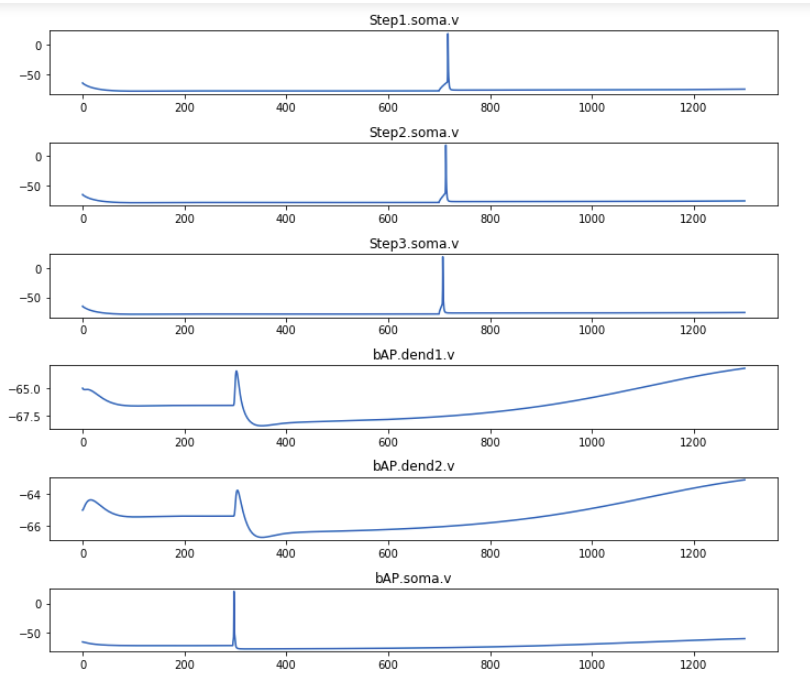
\includegraphics{figures/l5pc}
    \caption[Behavior of the L5PC model under optimized parameters]{Behavior of the L5PC model is explored under only one stimulus strength. Membrane potential this time is viewed from recording locations in the soma and dendrites}
    \label{fig:after_optimization}
\end{figure}

\begin{figure}
    \centering
    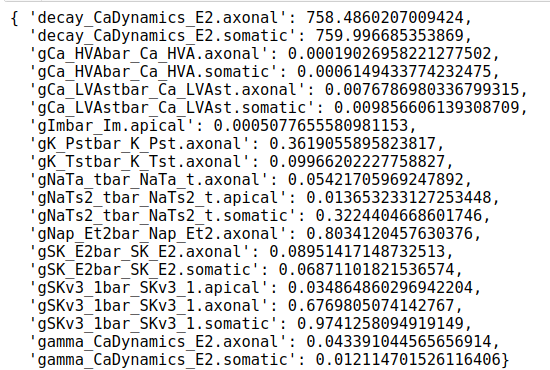
\includegraphics{figures/parameters_opt_l5pc.png}
    \caption{Caption}
    \label{fig:ca1_parameters}
\end{figure}




\begin{figure}
\begin{center}
\centering
\begin{subfigure}%{.2\textwidth}
  \centering
   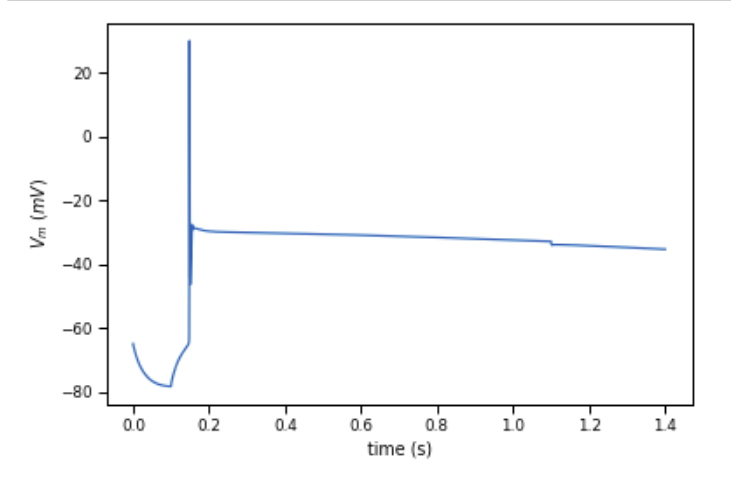
\includegraphics[scale=0.8]{figures/correct_active_l5pc.png}
    \caption{A current injection sufficient for causing a single spike is applied for a whole second from $100ms-1100ms$}
  \label{fig:sub1}
\end{subfigure}

As a reference point for understanding 
    \caption{The spike shape is very brief in duration, and so it is worth zooming in for a closer look}

\centering
\begin{subfigure}%{.2\textwidth}
  \centering
    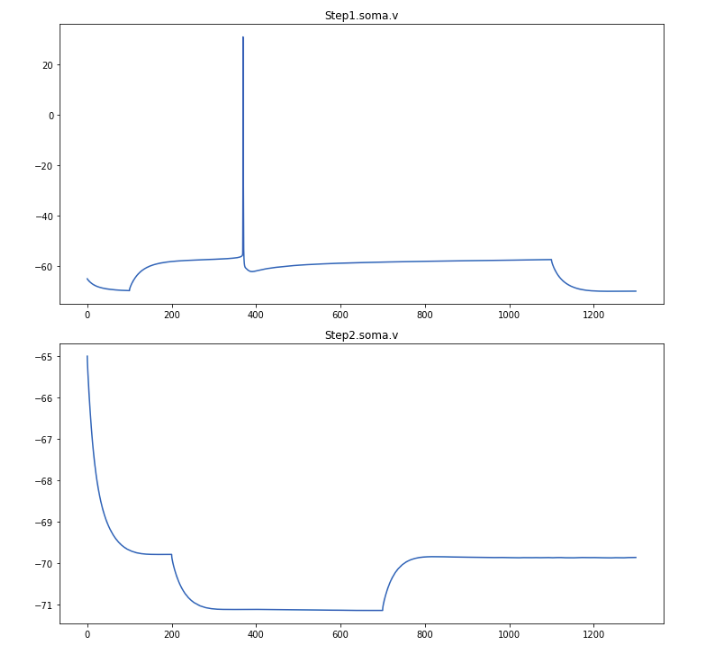
\includegraphics[scale=0.8]{figures/L5Somatosensory_not_optimized.png}
    \caption[SHORT CAPTION]{$V_{m}$ in $(mV)$ versus time $ms$, plots include a suprathreshold (top) and subthreshold stimulus (below)}
  \label{fig:brief_shape}
\end{subfigure}

\centering
\begin{subfigure}%{.2\textwidth}
  \centering
    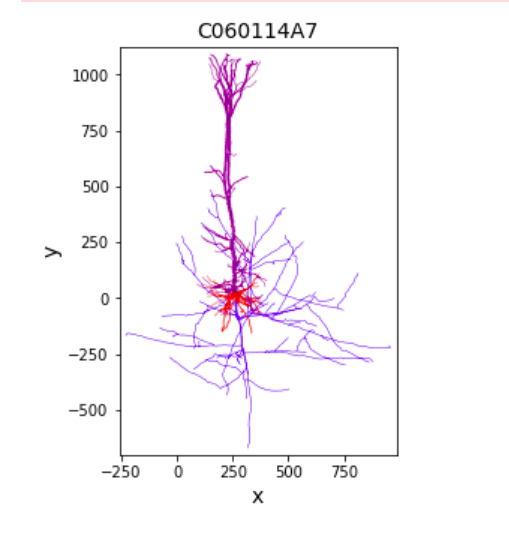
\includegraphics[scale=0.8]{figures/morphology_view.png}
    \caption[SHORT CAPTION]{This multi-compartment model is spatially extended, so a 2D depiction of its 3D form is warranted.}
  \label{fig:brief_shape}
\end{subfigure}

\begin{subfigure}%{.2\textwidth}
  \centering
    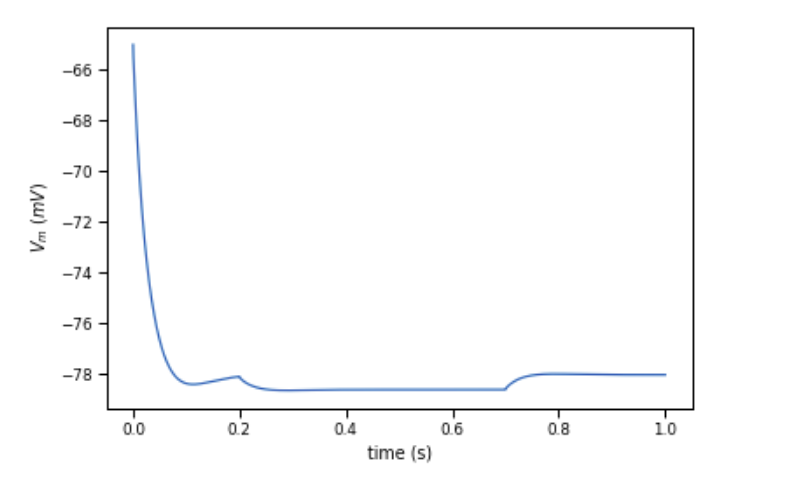
\includegraphics[scale=0.8]{figures/correct_passive_l5pc.png}
    \caption{A current injection value of -$10pA$ is applied to the cell for the duration of $200ms-700ms$}
  \label{fig:passive_properties_fine}
\end{subfigure}
\label{fig:test}
\end{center}
\end{figure}



A test suite was constructed using NeuroElectro for the non specific [cortical regions] layer 4/5 cortex pyramidal cell, and we were able to evaluate this layer 5 PC cells against the criteria of the neuroelectro test suite. Note the unnatural looking brief spike duration of the model cell spike  \ref{fig:brief_shape}. It is possible that the majority neuroelectro experiments on the layer 5 pyramidal cell were conducted under room temperature as opposed to body temperature, as there is evidence that the temperature of cortical tissue modulates spike width \cite{goldin2017temperature}, in particular cooling can contract their spike width

%%
% https://neuroelectro.org/data_table/36261/
%%
% from spike width table: 0.65 ± 0.13	1.04 ± 0.25**	0.51 ± 0.03**	0.59 ± 0.06	0.61 ± 0.03
%%
%
\caption[Observed and Predicted L5PC]{Observations, predictions, and Z-scores pertaining to the NeuronUnit-optimized Layer 5 Pyramidal Neuron}
\label{tab:l5pc_table}
\end{table}

Due to computational limitations this model was only run for 
$12$ offspring, and $30$ generation. Actually a minimum of $\mu=100$, $NGEN =100$ was prescribed by the scientists who optimized the initial model, however such a large compute job required prohibitive computational resources.

The unoptimized model had statistics:
$(\chi^{2},p_{value})=(13.56, 0.094)$

The optimized model produced statistics
$(\chi^{2},p_{value})=(6.63, 0.57)$

Optimization then clearly improves the model, however, it does not bring the model  biological plausibity.
This can be improved by omitting some of the worst tests, overall, the tests are compromized.



It is worth noting that the layer 5 neocortical pyramidal neuron was very slow to dispatch relative to the reduced models developed in this thesis work. Where as a typical reduced model described here evaluated in the order of $~0.0025 seconds$, this model on average took $5.74$, for a single run and $34.8$ to solve for the models Rheobase, current.

This model was pre-optimized to fit to spike times and F/I mainly, and so it should not necassarily be expected to fit other electrical charactersistics of the cell. Only the rheobase test, and the time constant test seemed to fall within the range of biological plausibility.
None the less, this model remains a useful benchmark for reduced neuronal models.